\begin{frame}
\frametitle{The Variational Formulation}
    \begin{block}{The Abstract Variational Formulation}
        Find $u_{\mathcal{F}} \in \H_{\mathcal{F}}$ such that
        \begin{align}
        \label{eq:directH1}
            b\left(u_{\mathcal{F}},\phi_{\mathcal{F}}\right) = f\left(\phi_{\mathcal{F}}\right), \quad \forall \phi_{\mathcal{F}} \in \H_{\mathcal{F}},
        \end{align}
        where:
        \begin{itemize}
            \item $f(\cdot)$ is a linear form,
            \item $b$ represents a bilinear form defined on $\H \times \H$,
            \item $\H_{\mathcal{F}} \coloneqq \textrm{span}\{\phi_{1}, \dots, \phi_{n_{\mathcal{F}}}\}$ denotes the finite element space,
            \item $\mathcal{T}$ represents the discretization of $\H$ into finite elements, where $\H_{\mathcal{F}} \subset \H$,
            \item $\mathcal{F} = \{\phi_{i}\}_{i=1}^{n_{\mathcal{F}}}$ is the set of basis functions defining $\H_{\mathcal{F}}$,
            \item $n_{\mathcal{F}}$ is the dimension of $\H_{\mathcal{F}}$, i.e., $n_{\mathcal{F}} = \textrm{dim}(\H_{\mathcal{F}})$,
            \item $u_{\mathcal{F}}$ is the Galerkin approximation of $u$ within $\H_{\mathcal{F}}$.
        \end{itemize}
    \end{block}     
\end{frame}

\begin{frame}
\frametitle{Basis Function Decomposition}
    \begin{block}{Decomposition into Essential and Removable Basis Functions}
        For any element $K$, consider the following sets and spaces:
        \begin{itemize}
            \item $\mathcal{R}_K$: the set of \emph{removable} basis functions associated to $K$ and $\abs{\mathcal{R}_K}$ its cardinality.
            \item $\H_{\mathcal{R}_K}$: the space generated by $\mathcal{R}_K$.
            \item $\mathcal{E}_K \coloneqq \mathcal{F} \setminus \mathcal{R}_K$: the set of \emph{essential} basis functions.
            \item $\H_{\mathcal{E}_K}$: the space associated with $\mathcal{E}_K$.
        \end{itemize}

        % Additional items can be uncommented and added here if needed
    \end{block}
    These satisfy the following properties:

    \begin{center}
        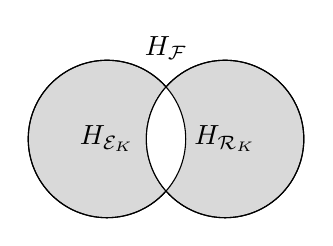
\begin{tikzpicture}
            % First circle
            \node[circle, draw, fill=gray!30, minimum size=2cm, label=center:\( H_{\mathcal{E}_K} \)] (HEK) at (0,0) {};

            % Second circle
            \node[circle, draw, fill=gray!30, minimum size=2cm, label=center:\( H_{\mathcal{R}_K} \)] (HRK) at (1.5,0) {};

            % Overlap drawing with white intersection
            \begin{scope}
                \clip (0,0) circle (1cm);
                \fill[white] (1.5,0) circle (1cm);
            \end{scope}

            % Redraw the circle borders to ensure they are visible
            \draw (0,0) circle (1cm);
            \draw (1.5,0) circle (1cm);

            % Label for the gray area moved above the intersection
            \node at (0.75,1.15) {\( H_{\mathcal{F}} \)};
        \end{tikzpicture}
    \end{center}
    %        \begin{itemize}
    %            \item $\H_{\mathcal{E}_K} \subset \H_{\mathcal{F}}$ and $\H_{\mathcal{R}_K} \subset \H_{\mathcal{F}}$.
    %            \item $\H_{\mathcal{F}} = \H_{\mathcal{E}_K} \cup \H_{\mathcal{R}_K}$ with $\H_{\mathcal{E}_K}\cap \H_{\mathcal{R}_K} = \emptyset$.
    %        \end{itemize}
\end{frame}

\begin{frame}
\frametitle{Projection Operator}
    \begin{block}{Definition of the Projection Operator}
        For a given subset of basis functions $\mathcal{S} \subset \mathcal{F}$ that generates the space $\H_{\mathcal{S}} \subset \H_{\mathcal{F}}$, we define our \emph{projection operator} $\Pi_{\mathcal{F}}^{\mathcal{S}}$: $\H _{\mathcal{F}} \longrightarrow \H_{\mathcal{S}}$ as
        \begin{equation}
            \Pi_{\mathcal{F}}^{\mathcal{S}} u_{\mathcal{F}} \coloneqq \sum_{\phi_{i} \in \mathcal{S}} u_{i} \phi_{i},
        \end{equation}
        where we extract the coefficients of $u_{\mathcal{F}}$ corresponding to the basis functions in $\mathcal{S}$, and we set the others to zero.
    \end{block}
    Hence, any function $u_{\mathcal{F}} \in \H_{\mathcal{F}}$ can be decomposed as:
        \begin{equation}
            u_{\mathcal{F}} =  \Pi_{\mathcal{F}}^{\mathcal{E}_K} u_{\mathcal{F}} + \Pi_{\mathcal{F}}^{\mathcal{R}_K} u_{\mathcal{F}}.\label{eq:decomposition}
        \end{equation}

        Note: For a single mesh, the solution $u_{\mathcal{E}_K}$ in $\mathcal{E}_K$ associated with Equation~\eqref{eq:decomposition} is not computed explicitly. Instead, the projection of $u_{\mathcal{F}}$ onto $\mathcal{E}_K$ is used to approximate it.

\end{frame}

\begin{frame}{Error indicators in our Strategy}

Let $\norm{\cdot}_e$ be the \emph{energy norm} associated with the Hilbert space $\H$. \\

\textbf{For Elliptic Problems:}
The energy norm is defined from the bilinear form of the problem $b$, that is, 
\[\norm{\cdot}_e^2 = b\left(\cdot, \cdot\right).\]

\textbf{For Non-Elliptic Problems:}
We define an alternative operator $a$, not necessarily the original bilinear form, such that 
\[\abs{b\left(\phi, \psi\right)} \leq \abs{a\left(\phi, \psi\right)}, \, \forall \phi, \psi \in \H\]
and the energy norm is 
\[\norm{\cdot}_e^2 = a\left(\cdot, \cdot\right).\]

The choice of these operators might highly influence the results of the adaptive process, an essential ingredient of adaptive strategies.

\end{frame}

\begin{frame}{Energy-norm based Elliptic Problems}

For a given element $K \in \mathcal{T}$, our goal is to quantify the energy lost in the solution when removing a subset of basis functions from the set of \emph{removable} basis functions $\mathcal{R}_K$. % Specifically, we compute:
\[\norm{u_{\mathcal{F}} - u_{\mathcal{E}_K}}_e^2.\]
%Note: A small value indicates that the energy of the removed basis functions is insignificant, suggesting comparable results between fine and unrefined meshes.

\textbf{Mathematical Derivation:} Analogously to Cea's lemma proof, we derive:
\begin{align}
  \norm{u_{\mathcal{F}}-u_{\mathcal{E}_K}}_e^2 &= b\left(u_{\mathcal{F}}-u_{\mathcal{E}_K},u_{\mathcal{F}}-u_{\mathcal{E}_K}\right) \\
  &= b\left(u_{\mathcal{F}}-u_{\mathcal{E}_K},u_{\mathcal{F}}-\Pi_{\mathcal{F}}^{\mathcal{E}_K} u_{\mathcal{F}}\right) + b\left(u_{\mathcal{F}}-u_{\mathcal{E}_K},\Pi_{\mathcal{F}}^{\mathcal{E}_K}u_{\mathcal{F}}-u_{\mathcal{E}_K}\right) \\
  &\leq \norm{u_{\mathcal{F}}-u_{\mathcal{E}_K}}_{e}\norm{u_{\mathcal{F}}-\Pi_{\mathcal{F}}^{\mathcal{E}_K}u_{\mathcal{F}}}_e,
\end{align}
where we use the $b$-orthogonality of $u_{\mathcal{F}}-u_{\mathcal{E}_K}$ with $\H_{\mathcal{E}_K}$ and the Cauchy-Schwarz inequality. Hence,
\begin{equation}
  \norm{u_{\mathcal{F}}-u_{\mathcal{E}_K}}_e \leq \norm{u_{\mathcal{F}}-\Pi_{\mathcal{F}}^{\mathcal{E}_K} u_{\mathcal{F}}}_e=\norm{\Pi_{\mathcal{F}}^{\mathcal{R}_K} u_{\mathcal{F}}}_e. \label{eq:upperboundSPD}
\end{equation}

\textbf{Error Indicator:} We define the element-wise error indicator as
\begin{equation}
  \eta_K\coloneqq \norm{\Pi_{\mathcal{F}}^{\mathcal{R}_K} u_{\mathcal{F}}}_e^2, \quad \forall K \in \mathcal{T}.\label{eq:SPDindicators}
\end{equation}

\end{frame}

\begin{frame}{Energy-Based Non-Elliptic Problems}

  \textbf{Discrete Inf-Sup Condition:} We assume that $b$ satisfies the discrete inf-sup condition:
      %\item Existence of a positive constant $\gamma$ such that
      \begin{equation}
        \exists \, \gamma > 0, \quad \inf_{\phi \in \H_{\mathcal{E}_K}}\sup_{\psi \in \H_{\mathcal{E}_K}}\frac{b\left(\phi, \psi\right)}{\norm{\phi}_{e}\norm{\psi}_{e}} \geq \gamma.
        \label{eq:infsup}
      \end{equation}

  \textbf{Utilizing $b$-Orthogonality:} We use the $b$-orthogonality of $u_{\mathcal{F}}-u_{\mathcal{E}_K}$ with respect to $\H_{\mathcal{E}_K}$.
      %\item This allows control of $\norm{\Pi_{\mathcal{F}}^{\mathcal{E}_K}u_{\mathcal{F}}-u_{\mathcal{E}_K}}_e$:
      \begin{align}
        \gamma\norm{\Pi_{\mathcal{F}}^{\mathcal{E}_K}u_{\mathcal{F}}-u_{\mathcal{E}_K}}_e & \leq \sup_{\psi \in \H_{\mathcal{E}_K}}\frac{b\left(\Pi_{\mathcal{F}}^{\mathcal{E}_K}u_{\mathcal{F}}-u_{\mathcal{E}_K}, \psi\right)}{\norm{\psi}_{e}} \\
        & \leq M_b \norm{u_{\mathcal{F}}-\Pi_{\mathcal{F}}^{\mathcal{E}_K}u_{\mathcal{F}}}_e,
      \end{align}
      where $M_b$ is the continuity constant of $b$.

  \textbf{Concluding Inequality:} Hence, we derive the following bound:
      \begin{equation}
        \norm{u_{\mathcal{F}}-u_{\mathcal{E}_K}}_e^2 \lesssim \norm{u_{\mathcal{F}}-\Pi_{\mathcal{F}}^{\mathcal{E}_K}u_{\mathcal{F}}}_e^2=\norm{\Pi_{\mathcal{F}}^{\mathcal{R}_K}u_{\mathcal{F}}}_e^2.
        \label{eq:en_ne_bound}
      \end{equation}

\end{frame}

\begin{frame}
\frametitle{Extension to Goal-Oriented Adaptivity}
    \begin{block}{The Adjoint Problem}
        Find $v_{\mathcal{F}}\in \H_{\mathcal{F}}$ such that
  	\begin{align}
    	\label{eq:adjointH}
    	b\left(\phi_{\mathcal{F}},v_{\mathcal{F}}\right)=l\left(\phi_{\mathcal{F}}\right), \quad \forall \phi_{\mathcal{F}} \in \H_{\mathcal{F}},
  	\end{align}
        where:
        \begin{itemize}
            \item the objective is to produce a space $\H_{\mathcal{F}}$ with minimal dimension such that the error in the Quantity of Interest (QoI) is below a user-defined tolerance,
            \item the QoI of the solution $u_{\mathcal{F}}$ is expressed as $l(u_{\mathcal{F}})$,
            \item $v_{\mathcal{F}}$ is the Galerkin approximation of $v$ within $\H_{\mathcal{F}}$,
            \item $v_{\mathcal{E}_K}$ in $\mathcal{E}_K$ is considered for analysis purposes, but not computed in practice.
        \end{itemize}
    \end{block}     
\end{frame}

\begin{frame}{Quantifying Changes in the Quantity of Interest (QoI)}

For a given element $K \in \mathcal{T}$, we control $\abs{l\left(u_{\mathcal{F}}\right)-l\left(u_{\mathcal{E}_K}\right)}, \; \forall K \in \mathcal{T}$. 

% we aim to quantify the change in the QoI when removing some basis functions from $\mathcal{R}_K$ associated with $K$. 
\textbf{Using Galerkin Orthogonality:}
Since $\H_{\mathcal{E}_K} \subset \H_{\mathcal{F}}$, we have
\begin{equation}
  b\left(u_{\mathcal{F}}-u_{\mathcal{E}_K}, \phi\right)=0, \quad \forall \phi \in \H_{\mathcal{E}_K}.
\end{equation}

\textbf{Decomposing the Change in QoI:}
\begin{align}
  l\left(u_{\mathcal{F}}\right)-l\left(u_{\mathcal{E}_K}\right) & = b\left(u_{\mathcal{F}}-u_{\mathcal{E}_K},v_{\mathcal{F}}-v_{\mathcal{E}_K}\right) \\
  & = b\left(u_{\mathcal{F}}-u_{\mathcal{E}_K},\Pi_{\mathcal{F}}^{\mathcal{R}_K} v_{\mathcal{F}}\right) \quad (\text{second term vanishes})
\end{align}

\textbf{Applying Decomposition and Orthogonality:}
\begin{equation}
  \abs{l\left(u_{\mathcal{F}}\right)-l\left(u_{\mathcal{E}_K}\right)} \simeq \abs{b\left(\Pi_{\mathcal{F}}^{\mathcal{R}_K} u_{\mathcal{F}},\Pi_{\mathcal{F}}^{\mathcal{R}_K} v_{\mathcal{F}}\right)}
  \leq  \abs{a\left(\Pi_{\mathcal{F}}^{\mathcal{R}_K} u_{\mathcal{F}},\Pi_{\mathcal{F}}^{\mathcal{R}_K} v_{\mathcal{F}}\right)}.
\end{equation}

\textbf{Defining Element-wise Indicators:}
\begin{equation}
  \eta_K \coloneqq \abs{a\left(\Pi_{\mathcal{F}}^{\mathcal{R}_K} u_{\mathcal{F}},\Pi_{\mathcal{F}}^{\mathcal{R}_K} v_{\mathcal{F}}\right)}, \quad \forall K \in \mathcal{T}.
\end{equation}

\end{frame}

\begin{frame}
\frametitle{Error Indicators Using a Pseudo-Dual Operator}
    \begin{block}{The Adjoint Problem}
        Find $\te$ such that
      \begin{equation}
         \hat{b}\left(\phi_{\mathcal{F}},\te\right)=l\left(\phi_{\mathcal{F}}\right) - b\left(\phi_{\mathcal{F}},\Pi_{\mathcal{F}}^{\mathcal{E}_K} v_{\mathcal{F}}\right), \quad \forall \phi \in \mathcal{H},
        \label{eq:forward_e}
      \end{equation}
        with the following specifications:
        \begin{itemize}
            \item $\eta_K$ is defined as the error indicator associated with the element $K$
             \begin{equation}
        		\eta_K \coloneqq \abs{\hat{b}\left(\Pi_{\mathcal{F}}^{\mathcal{R}_K} u_{\mathcal{F}}, \te\right)}, \quad \forall K \in \mathcal{T},
       		\label{eq:1DGOAupperbound}
     	   \end{equation}
            \item where, the operator $a\left(\cdot ,\cdot\right)$ is defined as $a\left(\cdot ,\cdot\right) = \hat{b}\left(\cdot ,\cdot\right)$.
        \end{itemize}
    \end{block}     
    \begin{thebibliography}{}
    \beamertemplatearticlebibitems
   \bibitem{darrigrand2020painless}
		V. Darrigrand, D. Pardo, I. Muga
		\newblock Goal-oriented adaptivity using unconventional error representations for the 1D Helmholtz equation
		\newblock \emph{Computers \& Mathematics with Applications}, 2015
    \end{thebibliography}
\end{frame}